\section{Introduction}\label{introduction}

The Internet of Things (IoT) has become the primary attack surface for network intrusions, and machine-learned intrusion detection systems (IDS) are now standard components of IoT security stacks \citep{ref1,ref2}. As these models have grown more capable, they have also grown more opaque, and explainable AI (XAI) has been proposed as the remedy: post-hoc attribution methods such as SHAP \citep{ref3} and LIME \citep{ref4} are routinely layered onto IoT-IDS classifiers to justify their decisions to operators, auditors, and regulators \citep{ref5,ref6}. A 2026 state-of-the-art survey by Karras et al.~\citep{ref1} (the direct point of departure for this paper) synthesizes this literature and identifies a \emph{resource--interpretability gap}: computationally intensive explainers are applied on constrained edge and federated platforms without the explanation cost itself being measured against the device's actual latency, memory, or energy budget. An independent, contemporaneous evidence synthesis spanning more than 200 papers \citep{ref7} converges on the same diagnosis from a different direction: the field has weak evidence that IoT-edge explanations are faithful, robust, or deployable, because most studies validate on static benchmark datasets rather than live or adversarial conditions, and rely almost exclusively on SHAP and LIME, methods imported from generic tabular machine learning rather than designed for temporal, relational network telemetry.

Both sources converge on a second, sharper point. Karras et al.~\citep{ref1} formalize a hardware-centric evaluation framework (the Computational Complexity Score (CCS), Memory Footprint Ratio (MFR), Temporal Coherence (TC), and a Unified Multi-Criteria Evaluation Framework for IoT (UMCEF\_IoT) that aggregates fidelity, efficiency, robustness, and sparsity into one composite score), but these metrics are defined by equation and never computed on real IoT traffic in that survey, nor, to our knowledge, anywhere else in the literature we were able to locate. The evidence synthesis \citep{ref7} independently lists two open research questions that this gap leaves unanswered: (i) \emph{how can explanations be made faithful, low-latency, and adversarially robust on heterogeneous edge hardware?}, and (ii) \emph{what network-native XAI methods best explain temporal, relational, multi-protocol IoT traffic, given that most work still adapts generic SHAP or LIME rather than causal, graph-based, or protocol-aware alternatives?}

This paper answers both questions with a single, reproducible empirical study and one new technique.

\textbf{Contribution 1: the benchmark.} We implement the full hardware-centric metric suite that Karras et al.~\citep{ref1} define but do not compute: CCS, MFR, TC, and the UMCEF\_IoT composite (their Equation 58), together with a deletion/insertion fidelity measure and a top-\emph{k} feature-overlap robustness measure, and apply them to four explainers (TreeSHAP, KernelSHAP, a lightweight/sparsified KernelSHAP variant, and LIME) across two edge-representative models (a LightGBM ensemble and a compact multilayer perceptron, under 5,000 parameters) under three simulated resource tiers calibrated to Raspberry Pi 4, Jetson Nano, and an unconstrained baseline. Each (explainer, model, tier) cell is measured inside an isolated, resource-capped subprocess so that a hard out-of-memory failure or allocator stall is recorded as data rather than crashing the experiment.

\textbf{Contribution 2: CC-SHAP.} Directly answering the field's call for causal, network-native explainers \citep{ref1,ref7}, we propose Causal-Consolidated SHAP (CC-SHAP): a post-processing layer, not a new attribution algorithm from scratch, that learns a bounded causal skeleton (a conditioning-set-limited PC-algorithm variant) over the training features once, offline, and at explanation time consolidates a base explainer's attribution mass onto the single strongest feature within each causally entangled cluster, rather than allowing it to be split ambiguously across correlated duplicates, a documented instability source for SHAP-family methods. Because the causal structure is learned once and reused, and the consolidation step itself is a cheap union-find pass, CC-SHAP's marginal cost over its base explainer is negligible.

\textbf{Contribution 3: adversarial comparability.} We implement both a single-step (FGSM) and a true iterative multiclass DeepFool attack, epsilon-clipped for comparability across a fixed perturbation budget, giving results directly comparable to the field's most-cited IoT-XAI robustness reference \citep{ref8}, alongside a black-box boundary attack for the non-differentiable tree ensemble.

\textbf{Contribution 4: cross-dataset replication.} We validate every finding twice: at production scale on CICIoT2023 \citep{ref9} (balanced 8-class grouping, 10,000 samples per class, 79,999 rows after data-quality correction) and again on Edge-IIoTset \citep{ref10} (15-class, 42-feature, duplicate-leakage-corrected), a structurally different dataset with a different class count, feature semantics, and data-quality profile. The result replicates on both: CC-SHAP is the most robust explainer of all five at every tested perturbation strength on both datasets, and by far the sparsest, trading a real but bounded fidelity cost for that gain.

The remainder of this paper is organized as follows. Section 2 reviews the IoT-edge XAI literature and positions our contribution against it. Section 3 details the datasets, models, explainers, the CC-SHAP technique, the resource-cap and adversarial harnesses, and the evaluation metrics. Section 4 reports results at production scale on both datasets. Section 5 discusses the findings, their limitations, and their implications. Section 6 concludes.

\begin{center}\rule{0.5\linewidth}{0.5pt}\end{center}

\section{Related Work}\label{related-work}

\subsection{XAI for IoT Intrusion Detection}\label{xai-for-iot-intrusion-detection}

Post-hoc, model-agnostic explainability has become the default approach for IoT-IDS because contemporary detectors rely on deep neural networks and ensemble methods whose predictive performance cannot be matched by inherently interpretable models (decision trees, linear models) without substantial accuracy loss \citep{ref1}. SHAP \citep{ref3} and LIME \citep{ref4} dominate this literature: Houda et al.~\citep{ref11} and Keshk et al.~\citep{ref12} use SHAP-based explanations to justify deep-learning IDS decisions; Moustafa et al.~\citep{ref13} survey explainable cyber-defence opportunities for IoT broadly. Ogunseyi et al.~\citep{ref14} formalize what they term the accuracy--efficiency--explainability trilemma in a systematic review of explainable deep-learning IDS, concluding that the three objectives are rarely optimized jointly. Karras et al.~\citep{ref1} extend this diagnosis into a full hardware-centric taxonomy spanning device, edge, and cloud deployment tiers, and is the survey this paper is a direct empirical companion to. A large and still-growing body of applied work instantiates single-system versions of this pattern, a detector paired with a post-hoc explainer evaluated on accuracy and a qualitative inspection of attributions rather than against a resource or robustness budget: Mohamed et al.'s APEX-IDS \citep{ref37} combines CNN--LSTM detection with SHAP and LIME across five benchmark datasets; Madhanraj's XAI-IoTIDS \citep{ref39} pairs Bayesian-optimized XGBoost with SHAP on CICIoT2023; Loi, Canavese, and Regano \citep{ref38} apply SHAP directly to an industrial-IoT IDS; Zhang et al.'s GBFKAN \citep{ref29} uses a Kolmogorov--Arnold network layer specifically to make a gated BiLSTM architecture's internal decision paths more inspectable, supplementing (rather than replacing) a post-hoc SHAP pass. None of these report explanation cost, memory footprint, or adversarial robustness alongside their accuracy numbers, the omission this paper's benchmark is designed to close.

\subsection{Federated, Lightweight, and Resource-Aware Explainability}\label{federated-lightweight-and-resource-aware-explainability}

A second strand of the literature moves XAI into federated and split-learning architectures to preserve privacy while explaining distributed models \citep{ref1,ref15,ref16}. Zhao et al.~\citep{ref17} report a split federated IDS for consumer healthcare achieving millisecond-scale inference but acknowledge substantial per-round communication overhead for the accompanying explanations; Singh and Roy \citep{ref18} reframe explanation as a system service (Explainability-as-a-Service) with caching and adaptive delivery, reporting a 38\% latency reduction across edge use cases. Nassef et al.~\citep{ref19} target lightweight, energy-aware intrusion detection for industrial IoT using TinyML. Narkedimilli et al.'s FedGuard-IIoT \citep{ref45} and Elsayed, Zamzam, and Ashour's federated IIoT-IDS \citep{ref46} both report that centralized training outperforms federated variants on raw accuracy (the latter study: 97.7\% centralized vs.~95\% federated on Edge-IIoTset) while arguing the federated route is still preferable once privacy and client-heterogeneity constraints are counted, a trade-off reported qualitatively rather than folded into a single comparable score, which is exactly the role the UMCEF\_IoT composite (Section 3.6) is designed to play. On the model-compression side, Umair et al.~\citep{ref27} distill a teacher IDS into a lightweight student (263k to 120k parameters, 1.00 MB to 471.67 KB) and confirm with SHAP that the distilled model retains the teacher's key feature attributions, compressing the \emph{model} rather than the \emph{explanation}, a complementary axis to this paper's focus on explainer-side cost. Kalpana and Jayalakshmi \citep{ref28} report a SHAP-explained LSTM-CatBoost hybrid for CICIoT2023 with edge quantization cutting model size by 94.1\% and latency by 86.2\%, again without reporting the explanation call's own cost against that shrunken latency budget. Across this literature, the recurring finding is that explanation cost is measured inconsistently or not at all relative to the hardware budget it must fit. That is precisely the gap Karras et al.~\citep{ref1} formalize and that we close empirically in Section 4.

\subsection{Evaluation Rigor and the Case for Causal, Network-Native Explainers}\label{evaluation-rigor-and-the-case-for-causal-network-native-explainers}

Several recent evaluation studies find that predictive accuracy does not imply explanation fidelity: Kalakoti et al.~\citep{ref20} report a systematic, quantitative evaluation of explainer fidelity for IoT botnet detection, finding substantial variation in faithfulness among explainers that perform similarly on raw accuracy. Munilla and Khammas \citep{ref8} test explanation stability under DeepFool adversarial perturbation against DNN-based IoT-IDS and find explanations are frequently more fragile than the underlying model's predictions, the specific robustness protocol we replicate and extend in Section 3.4. Nascita et al.~\citep{ref22}, surveying explainable AI for internet traffic classification and intrusion detection, argue explicitly that methods imported from tabular machine learning are not tailored to the temporal, relational structure of network telemetry, and call for causal, graph-based, or protocol-aware alternatives, a call echoed independently by the evidence synthesis underlying this paper \citep{ref7} and by the ``Causal Semantics'' pillar Karras et al.~\citep{ref1} list among three unaddressed transformative research frontiers in their own survey's forward-looking discussion. A small number of recent studies move toward graph-structured alternatives without adopting a causal framing specifically: Kumar et al.~\citep{ref30} pair a graph neural network with an attention mechanism and federated training for edge intrusion detection on Edge-IIoTset and TON\_IoT, and report the GNN's attention weights as a qualitative explanation surface, while O'Shea et al.~\citep{ref31}, outside the IoT-IDS domain but methodologically adjacent, use explainable graph ensemble learning for multivariate time-series anomaly detection in cloud microservices. Neither work constructs an explicit causal graph over the feature space or quantifies how structure-aware attribution compares to generic SHAP/LIME under a matched robustness protocol. To our knowledge, no prior IoT-edge XAI study has implemented and evaluated a causal explainer against this exact resource-aware, adversarially-tested protocol; CC-SHAP (Section 3.3) is proposed to close that gap directly.

\subsection{Adversarial Robustness of Explanations}\label{adversarial-robustness-of-explanations}

A distinct and smaller literature treats the explanation itself, rather than the underlying classifier, as the object under adversarial attack or adversarial defense. Sharma et al.~\citep{ref33} invert the usual direction of use, employing SHAP \emph{DeepExplainer} attribution fingerprints as a detector of adversarially perturbed inputs rather than as an end-user-facing explanation, reporting that subtle shifts in per-feature attribution reliably flag evasion attempts that the classifier alone misses. Zhang et al.'s NonsaliencyCrossover \citep{ref32} generates black-box adversarial examples by crossing over the \emph{non-salient} (low-attribution) portion of one traffic sample into another, explicitly exploiting the sparsity structure an explainer reveals to construct attacks more query-efficient than six state-of-the-art baselines, a finding with a direct implication for this paper's own adversarial protocol (Section 3.5): an explainer's sparsity pattern is not merely a usability property but a potential attack surface, a tension we return to in Section 5.4. Du et al.~\citep{ref34} combine ensemble adversarial training with explanation-based resilience diagnostics as a joint defense layer for AI-powered IDS, evaluating evasion-attack survivability rather than deletion/insertion fidelity. None of these three studies reports the \emph{computational} cost of the explanation-robustness pipeline itself against an edge resource budget, which is where the present paper's contribution is positioned relative to this group: we treat adversarial robustness of the explanation as one axis of a four-axis composite (fidelity, efficiency, robustness, sparsity) rather than as a standalone defense mechanism.

\subsection{Evaluation Frameworks for IoT/IIoT XAI}\label{evaluation-frameworks-for-iotiiot-xai}

A parallel thread of work builds general-purpose evaluation frameworks for XAI methods rather than proposing a new explainer. Abdallah et al.'s E-XAI \citep{ref35} evaluates SHAP and LIME as black-box explainers across seven AI methods and three network-intrusion datasets along six metrics (descriptive accuracy, sparsity, stability, efficiency, robustness, and completeness), a metric vocabulary that substantially overlaps with, but does not include, the hardware-centric CCS/MFR pairing this paper computes. Gummadi et al.'s E-RXAI-IoT \citep{ref21} runs a comparable seven-metric evaluation specifically for \emph{rule-based} XAI methods (Anchor, RuleFit) across two IoT anomaly-detection datasets, finding that rule-based explainers' interpretability advantage comes with measurable fidelity and coverage trade-offs against the post-hoc SHAP/LIME family this paper benchmarks. Sathvik and Saini's survey \citep{ref36} of 21 trustworthy-AI papers identifies what they term a ``privacy--transparency paradox'' (explanations detailed enough to earn operator trust also expose the decision boundary to model-inversion attack) and surveys compact distillation frameworks and attribution fingerprinting (cf.~\citep{ref27,ref33}) as partial responses. None of these frameworks evaluates explainers under a simulated edge resource cap with isolated per-cell measurement, which is the specific methodological contribution Section 3.4's harness makes to this line of work.

\subsection{Applied SHAP/LIME Systems Across IoT and IIoT Domains}\label{applied-shaplime-systems-across-iot-and-iiot-domains}

Beyond the evaluation-focused studies above, a broad applied literature deploys SHAP or LIME as a fixed, un-interrogated component inside a larger detection pipeline, typically reporting accuracy and a qualitative attribution plot rather than any of the dimensions this paper measures. Representative recent examples include Saiyed and Al-Anbagi's HEAD system \citep{ref40}, which uses the geometric mean of normalized SHAP and LIME scores for joint feature selection in DDoS detection for industrial IoT, and the same authors' interactive SHAP-explained DDoS detector for consumer IoT \citep{ref41}; Nwakanma et al.'s Tree-LIME approach for SCADA-edge intrusion detection \citep{ref42}; Joshi and Prakash's hybrid SHAP--fuzzy framework for IoT botnet detection \citep{ref43}, which uses SHAP attributions as inputs to a fuzzy-rule layer rather than as the end-user explanation directly; and Tewari's white-box IDS architecture \citep{ref44}, which argues for inherently interpretable models over post-hoc explanation of black-box ones, a position this paper's own Introduction (Section 1) notes as the minority view in a literature still dominated by the post-hoc SHAP/LIME default \citep{ref1}. This group of studies collectively illustrates the scale of the applied gap Karras et al.~\citep{ref1} and the evidence synthesis underlying this paper \citep{ref7} diagnose: dozens of systems ship a post-hoc explainer as a feature, essentially none measure what that explainer costs the device it runs on, or whether it survives the adversarial conditions the detector itself is built to withstand.

\subsection{Positioning This Paper}\label{positioning-this-paper}

Table~\ref{tab0} summarizes where the studies reviewed in Sections 2.1--2.6 sit relative to the four evaluation axes this paper's benchmark reports jointly (fidelity, efficiency/resource-cap, adversarial robustness, sparsity), and relative to its proposed explainer family (generic post-hoc SHAP/LIME vs.~causal or graph-structured). No reviewed study reports all four axes jointly, and only the two causal/graph-adjacent studies \citep{ref30,ref31} move away from generic tabular SHAP/LIME toward a structure-aware explainer, neither with a resource cap or adversarial test.

\begin{table}[H] \caption{Positioning of this paper against the closest prior IoT/IIoT-XAI literature, by evaluation axis and explainer family.\label{tab0}} \begin{adjustwidth}{-\extralength}{0cm} \begin{tabularx}{\fulllength}{LCCCCC} \toprule \textbf{Study} & \textbf{Fidelity} & \textbf{Resource cost} & \textbf{Adversarial robustness} & \textbf{Sparsity} & \textbf{Explainer family} \\ \midrule Karras et al. \citep{ref1} (survey; metrics formalized, not computed) & n/a & n/a & n/a & n/a & generic SHAP/LIME (surveyed) \\ Munilla \& Khammas \citep{ref8} & n/a & n/a & \checkmark & n/a & generic SHAP/LIME \\ Kalakoti et al. \citep{ref20} & \checkmark & n/a & n/a & n/a & generic SHAP/LIME \\ Gummadi et al. \citep{ref21} (E-RXAI-IoT) & \checkmark & partial (efficiency) & n/a & \checkmark & rule-based (Anchor, RuleFit) \\ Abdallah et al. \citep{ref35} (E-XAI) & \checkmark & partial (efficiency) & \checkmark & \checkmark & generic SHAP/LIME \\ Sharma et al. \citep{ref33} & n/a & n/a & \checkmark (as a detector) & n/a & generic SHAP \\ Kumar et al. \citep{ref30} & n/a & n/a & n/a & n/a & GNN + attention \\ Umair et al. \citep{ref27} & n/a & partial (model, not explainer) & n/a & n/a & generic SHAP \\ \textbf{This paper} & \textbf{\checkmark} & \textbf{\checkmark (CCS, MFR, simulated tiers)} & \textbf{\checkmark (FGSM, DeepFool, black-box)} & \textbf{\checkmark} & \textbf{generic SHAP/LIME + causal (CC-SHAP)} \\ \bottomrule \end{tabularx} \end{adjustwidth} \end{table}

\subsection{Datasets}\label{datasets}

CICIoT2023 \citep{ref9} is a large-scale, realistic IoT attack-traffic corpus spanning benign traffic and multiple attack families (DDoS, DoS, reconnaissance, web-based, brute-force, spoofing, and Mirai-derived traffic), released as per-category CSV files without a unified label column. Edge-IIoTset \citep{ref10} is a comparably scaled industrial-IoT corpus with Normal traffic and 14 attack categories drawn from a richer, protocol-level feature set (including MQTT, Modbus, HTTP, and DNS fields). Because Edge-IIoTset is one of this paper's two evaluation corpora (Section 3.1), two further studies merit specific mention for their direct bearing on its data quality. Kulrujiphat and Kulrujiphat \citep{ref47} survey AI-based attack-detection models built on Edge-IIoTset, concluding that feature-selection choices materially drive reported accuracy and that federated learning with local differential privacy is the field's preferred route to the dataset's privacy requirements, context relevant to why Section 2.2's federated-XAI studies gravitate toward this corpus. Dhaou \citep{ref23} shows that several Edge-IIoTset protocol-identity fields (e.g., \texttt{dns.qry.name.len}, \texttt{mqtt.topic}) are so strongly correlated with the attack label that a linear classifier alone achieves near-perfect separation on the uncontrolled feature set, a feature-level leakage distinct from, and compounding, the exact-duplicate row leakage we identify and correct empirically in Section 3.1 of our own pipeline, and the direct empirical basis for this paper's own leakage-control discipline on that corpus. Taken together, these findings (a documented data-quality issue in this dataset family generally, and Edge-IIoTset's specific feature-level leakage) mean any accuracy number reported on Edge-IIoTset without an explicit account of its row- and feature-level leakage controls should be read cautiously, a caveat we apply to our own Section 4.2 results.

\begin{center}\rule{0.5\linewidth}{0.5pt}\end{center}

\section{Materials and Methods}\label{materials-and-methods}

\subsection{Datasets and Preprocessing}\label{datasets-and-preprocessing}

\textbf{CICIoT2023.} We use the official per-category release (34 raw attack/benign subdirectories), grouped into the 8-class scheme most consistent with published CICIoT2023 benchmarks (Benign, DDoS, DoS, Mirai, Recon, Spoofing, Web, BruteForce), stratified-subsampled to 10,000 rows per \emph{grouped} class. During development we discovered that the naive implementation of this subsampling cap was applied per \emph{raw} subfolder rather than per final grouped label; since several grouped classes (DDoS, 12 raw subfolders; Web, 6; Recon, 5) aggregate many raw subfolders, this silently inflated those classes to several multiples of the intended 10,000-row cap while single-folder classes (Benign, BruteForce) remained correctly capped, a severe, undisclosed class imbalance that would have inflated accuracy on majority classes and biased every downstream metric. We corrected this by grouping raw subfolders by final label \emph{before} applying the per-class budget, verified the fix produces exactly balanced classes, and report only results from the corrected loader. A second, independent issue surfaced at the same stage: rate-style features (packets divided by a flow duration that occasionally rounds to zero) contain a small number of literal infinity values (1 of 80,000 rows in the final run) that crash standard-library feature scaling; we detect and drop affected rows with a logged warning rather than allowing a silent crash or silent \texttt{NaN} propagation. The final, corrected training set comprises 59,999 training and 20,000 test rows across 39 numeric flow features.

\textbf{Edge-IIoTset.} We use the official ``Selected dataset for ML and DL'' release (\texttt{ML-EdgeIIoT-dataset.csv}, 157,800 rows, 15 classes: Normal plus 14 attack types), with the \texttt{Attack\_type} column as the label and non-numeric/identifier columns dropped. Measuring the duplicate-row leakage issue directly on this release, we find 814 of 157,800 rows (0.5\%) are exact duplicates by feature value; we apply the general, conservative form of the correction documented for this class of dataset \citep{ref23}: dropping exact duplicates, keeping the first occurrence, before stratified subsampling and the train/test split, so that no duplicate pair can land on both sides of the split. Because two raw classes (MITM, Fingerprinting) contain fewer than 1,500 rows before correction, we cap all classes at 1,000 samples per class (rather than CICIoT2023's 10,000) so the comparison remains class-balanced; this yields 10,800 training and 3,600 test rows across 42 numeric features after the leakage fix and duplicate removal.

Both loaders apply standard z-score normalization fit on the training split only, and a stratified 75/25 train/test split.

Figure 1 summarizes the full pipeline described in the remainder of Section 3: both datasets feed a shared preprocessing step, two models, five explainers (four baselines plus CC-SHAP, the latter drawing on an offline-learned causal skeleton), the resource-cap and adversarial harnesses that wrap every (explainer, model, tier) cell, and the metrics/composite score reported in Section 4.

\begin{figure}[H] \centering 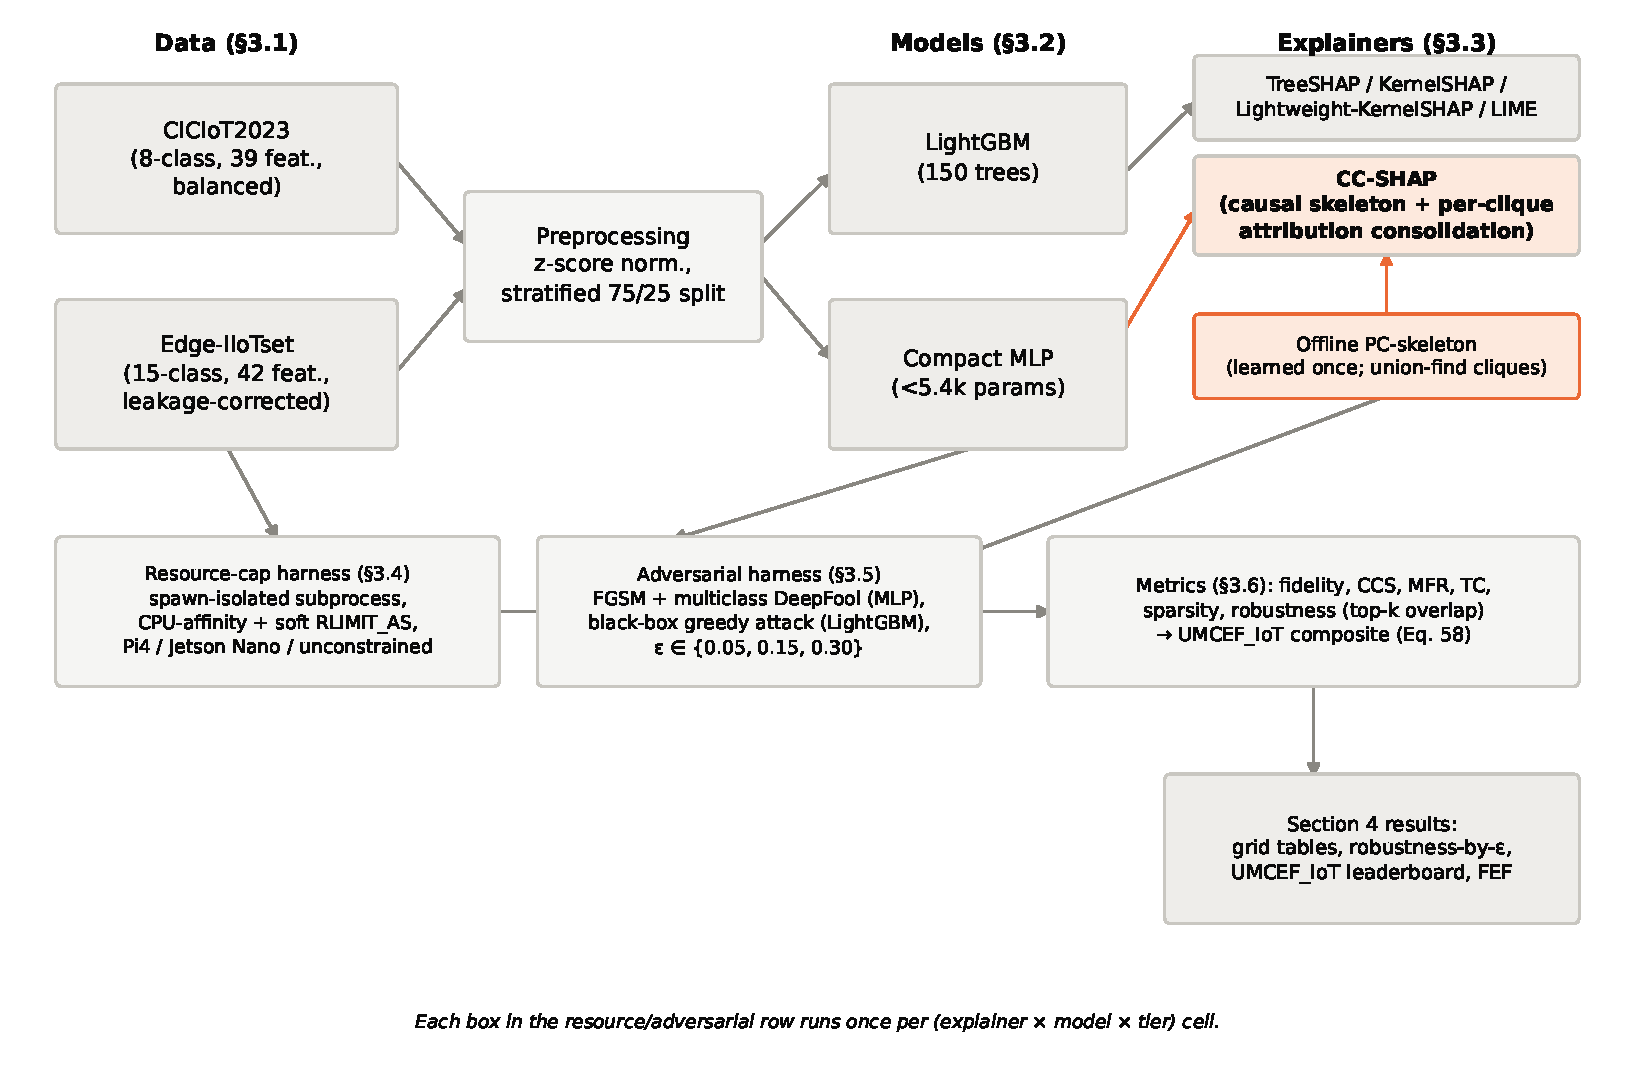
\includegraphics[width=0.95\textwidth]{results/figures/architecture.pdf} \caption{System architecture: data, models, explainers (including the CC-SHAP causal-skeleton sidecar), resource-cap and adversarial harnesses, and the metrics pipeline.\label{fig1}} \end{figure}

\subsection{Models}\label{models}

We train two models representative of the compute budgets actually available on IoT edge hardware, not research-scale architectures: (i) a LightGBM gradient-boosted ensemble (150 trees, max depth 6), chosen because its native tree structure admits exact TreeSHAP attribution; and (ii) a compact multilayer perceptron (two hidden layers, under 5,400 parameters in both experiments reported here (4,904 for CICIoT2023, 5,327 for Edge-IIoTset), trained with Adam for 30 epochs), representative of the small dense networks deployable on microcontroller-class hardware. Neither model is tuned for maximum accuracy; both are trained with fixed, reasonable defaults so that the explainer comparison is not confounded by per-model hyperparameter search.

\subsection{Explainers}\label{explainers}

Four established post-hoc explainers are benchmarked: \textbf{TreeSHAP} \citep{ref3}, the exact, polynomial-time SHAP variant available only for the tree ensemble; \textbf{KernelSHAP} \citep{ref3}, the model-agnostic baseline, applied to both models; a \textbf{lightweight KernelSHAP variant}, matching Table 23 of Karras et al.'s \citep{ref1} ``lightweight and sparsity-aware explainers'' research direction, implemented as KernelSHAP with a sharply reduced background-sample and coalition-sampling budget; and \textbf{LIME} \citep{ref4}, at its library-default 5,000-sample local-perturbation budget for all production-scale results reported here.

\subsubsection{CC-SHAP: Causal-Consolidated SHAP}\label{cc-shap-causal-consolidated-shap}

CC-SHAP is proposed as a fifth explainer and this paper's primary technical contribution. It operates in two stages.

\textbf{Offline, once:} a causal skeleton is learned over the training features using a conditioning-set-bounded variant of the PC algorithm \citep{ref24}. Standard PC-algorithm skeleton discovery tests pairwise conditional independence across conditioning sets of growing size, which is itself computationally expensive, the reason causal discovery is largely absent from resource-constrained IoT-XAI work to date. We deliberately bound the conditioning-set size to order $\leq$1 (marginal independence via Fisher-\emph{z} transform of the Pearson correlation, followed by a single round of conditioning on each other individual variable), which keeps skeleton discovery itself within a lightweight, edge-appropriate compute budget; this boundedness is a stated design choice, not a hidden simplification, and we quantify its cost directly (Section 4). The output is a symmetric adjacency matrix identifying feature pairs that remain plausibly directly dependent after this bounded test, which we decompose into connected components (``causally entangled cliques'') via union-find.

\textbf{At explanation time:} CC-SHAP takes attributions already produced by a base explainer (TreeSHAP for the LightGBM model, KernelSHAP for the multilayer perceptron, since no exact tree-structure attribution exists for a dense network) and, within each clique of the causal skeleton with more than one member, retains only the feature with the largest absolute attribution per sample, zeroing the rest. No additional model queries are made at this stage; the operation is a per-sample arg-max over each clique, which is why CC-SHAP's marginal latency over its base explainer is negligible (quantified in Section 4.1).

The rationale is that SHAP-family methods are documented to split attribution credit ambiguously across correlated features, a known source of explanation instability: the credit a redundant duplicate feature receives can differ between near-identical inputs or between runs using different background samples. CC-SHAP's hypothesis (formalized as H4 below) is that forcing attribution onto the single strongest signal in each entangled cluster should measurably increase sparsity and adversarial robustness, at a bounded, honestly reported cost to fidelity, not that it dominates on every metric simultaneously.

\textbf{Algorithm 1.} CC-SHAP (Causal-Consolidated SHAP).

\begin{verbatim}
Offline (once, over training set X, d features):
  1. For each feature pair (i, j): compute Fisher-z marginal independence test
     on Pearson r(X_i, X_j). If independence rejected at alpha, mark edge (i, j).
  2. For each surviving edge (i, j): re-test conditional independence of
     X_i, X_j given each single third variable X_k (k != i, j). If
     independence holds for any k, drop edge (i, j) (order-1 PC step).
  3. Build adjacency matrix A from the remaining edges.
  4. Decompose A into connected components C_1, ..., C_m via union-find
     ("causally entangled cliques").
  Output: clique assignment c: {1, ..., d} -> {1, ..., m}.

At explanation time (per explained sample x, base attribution vector phi(x)):
  1. For each clique C_r with |C_r| > 1:
       j* = argmax_{i in C_r} |phi_i(x)|
       for i in C_r, i != j*: phi_i(x) <- 0
  2. Return consolidated attribution phi'(x).
\end{verbatim}

\textbf{Complexity.} The offline step is O(d$^{2}$) marginal correlation tests plus O(d$^{2}$ $\cdot$ d) = O(d$^{3}$) in the worst case for the order-1 conditioning round (each of the O(d$^{2}$) surviving edges re-tested against up to d-2 conditioning variables); bounding the conditioning-set order at 1, rather than allowing the unbounded growth of the standard PC algorithm, is what keeps this from becoming exponential in d.~For the feature counts in this paper (d = 39 and d = 42), this is sub-second (Section 4.1: 1.01 s and 1.20 s respectively) and amortized over every subsequent explanation call, since it is computed once per dataset, not once per sample. The at-explanation-time step is O(d) per sample (a single pass over the clique assignment, each clique's arg-max computed in one pass over its members), strictly cheaper than a single additional model query, which is why CC-SHAP's marginal latency over its base explainer is negligible regardless of which base explainer it wraps.

\subsection{Resource-Cap Simulation}\label{resource-cap-simulation}

Each (explainer, model, resource-tier) combination is executed inside an isolated, freshly spawned subprocess rather than the parent experiment process, for two reasons. First, it allows a hard out-of-memory abort (observed in practice to originate from the native BLAS/OpenMP allocator rather than a catchable Python exception when memory pressure is severe) to be recorded as a result for that one cell rather than terminating the entire experiment. Second, it avoids a documented class of fork-safety hazard in which a multithreaded library (SHAP's KernelExplainer, or the progress-bar library's monitor thread) holds a lock at the moment of forking that can never be released in a forked child, causing a silent deadlock; we use the \texttt{spawn} process-start method with a picklable, top-level dispatch function rather than \texttt{fork}, after confirming this hazard empirically during development.

Three resource tiers are simulated via CPU-core affinity restriction and a soft virtual-memory ceiling (\texttt{RLIMIT\_AS}), calibrated to Raspberry Pi 4 (4 cores), Jetson Nano (4 cores), and an unconstrained development-machine baseline. We note, as an honest methodological limitation rather than an implementation detail, that in-process virtual-memory caps below approximately 1.5 GB proved unreliable in our own testing: the baseline footprint of a fresh Python interpreter with NumPy, LightGBM, PyTorch, and SHAP already imported can itself approach or exceed a literal 1 GB budget, causing the underlying native allocator to enter multi-second retry storms rather than failing cleanly. We therefore report simulated-tier results as \emph{relative} resource-cost comparisons across explainers (which method is cheaper than which other method under matched conditions), and explicitly recommend container-level (cgroup) enforcement, which uses the kernel out-of-memory killer and fails deterministically, as the authoritative path for any future claim of a literal absolute hardware budget.

\subsection{Adversarial Perturbation}\label{adversarial-perturbation}

Three attacks are used to test explanation robustness under input perturbation, chosen for correctness per model type rather than forcing one library across incompatible architectures. For the differentiable multilayer perceptron, we implement both the single-step Fast Gradient Sign Method (FGSM) and a true iterative multiclass DeepFool attack \citep{ref25} (the specific attack protocol used by the field's most-cited IoT-XAI adversarial-robustness reference \citep{ref8} against a DNN-based IDS) with the accumulated perturbation clipped to a fixed L-infinity epsilon ball at every iteration so results remain directly comparable to the FGSM sweep at matched epsilon values; this epsilon-clipping is an explicit, stated adaptation of literature-standard unbounded minimal-norm DeepFool, made for comparability, not a silent deviation. For the non-differentiable LightGBM ensemble, for which neither FGSM nor DeepFool applies, we implement a black-box greedy attack that perturbs the features a finite-difference sensitivity probe identifies as most influential, within the same epsilon budget. All results reported in Section 4 use DeepFool for the multilayer perceptron and the black-box attack for LightGBM, at epsilon $\in$ \{0.05, 0.15, 0.30\} in standardized-feature units.

\subsection{Evaluation Metrics}\label{evaluation-metrics}

\textbf{Fidelity} is measured via the standard deletion/insertion protocol: predicted-class probability is tracked as the top-attributed features are progressively masked out (deletion, expecting a fast collapse for a faithful explanation) or progressively restored from a baseline (insertion, expecting a fast rise), combined into a single {[}0,1{]} score:

\begin{equation}\mathrm{FID}(x) = \tfrac{1}{2} \left[ (1 - \mathrm{AUC}_{\mathrm{deletion}}(x)) + \mathrm{AUC}_{\mathrm{insertion}}(x) \right],\end{equation}

averaged across the explained sample batch, where AUC\_deletion and AUC\_insertion are the areas under the predicted-class-probability-vs-fraction-of-features-removed/restored curves.

\textbf{Computational Complexity Score (CCS)} and \textbf{Memory Footprint Ratio (MFR)} follow Karras et al.'s \citep{ref1} definitions. For explainer $\Phi$ in cell (model, tier):

\begin{equation}\mathrm{CCS}(\Phi) = t_{\min} / t(\Phi), \qquad \mathrm{MFR}(\Phi) = 1 - \left( m(\Phi) / M_{\mathrm{tier}} \right),\end{equation}

where t($\Phi$) is the cell's measured wall-clock explanation latency, t\_min is the fastest latency observed for that explainer across the tiers compared, m($\Phi$) is peak measured memory, and M\_tier is the simulated tier's memory budget; CCS is therefore bounded in (0, 1{]} with 1 denoting the fastest observed configuration, and MFR is higher when more of the tier's budget is left unused.

\textbf{Temporal Coherence (TC)} measures the rank-correlation stability of feature attributions across the explained batch, treated as a proxy sliding window of behaviorally adjacent samples (e.g., consecutive flows from the same source in a live deployment), rather than a per-sample quantity:

\begin{equation}\mathrm{TC} = \mathrm{clip}\!\left( \frac{\bar\rho + 1}{2}, 0, 1 \right), \quad \text{where } \bar\rho = \frac{1}{N-1} \sum_{i=1}^{N-1} \rho_{\mathrm{Spearman}}\!\left( \varphi(x_i), \varphi(x_{i+1}) \right),\end{equation}

for the \emph{N} explained samples x\_1, \ldots{}, x\_N in the order they were drawn, mapping the mean pairwise Spearman correlation from {[}-1, 1{]} to {[}0, 1{]} so that, consistent with every other metric in this paper, higher is better. We report one TC value per (explainer, model, tier) cell rather than per sample. This is a deliberate proxy, not a literal temporal ordering: the datasets used here (Section 3.1) are not temporally ordered flow sequences, so ``adjacent'' means adjacent in the explained-sample draw order, not adjacent in real time or in feature-space distance; a genuine temporal or nearest-neighbor-based TC is noted as future work (Section 5.5). As a proxy for whether explanations ``flicker'' between similar inputs, it is itself a form of the instability CC-SHAP is designed to reduce.

\textbf{Explanation robustness} is the top-\emph{k} feature-overlap (Jaccard-style) between an explanation computed on a clean input and the same explanation computed on its adversarially perturbed counterpart:

\begin{equation}\mathrm{ROB}_\varepsilon(x) = \frac{\left| \mathrm{top}_k(\varphi(x)) \cap \mathrm{top}_k(\varphi(x+\delta_\varepsilon)) \right|}{\left| \mathrm{top}_k(\varphi(x)) \cup \mathrm{top}_k(\varphi(x+\delta_\varepsilon)) \right|},\end{equation}

averaged across the explained sample batch and reported per epsilon, where $\delta$\_$\varepsilon$ is the attack-specific perturbation bounded at L-infinity radius $\varepsilon$, and \emph{k} = 5 throughout. We flag a specific interaction this fixed \emph{k} has with CC-SHAP: CC-SHAP's own sparsity (0.950 on CICIoT2023, roughly two non-zero features out of 39; Section 4.1) means its true active-feature count is typically smaller than \emph{k}, so three or four of the five ``top-\emph{k}'' slots for a CC-SHAP explanation are zero-valued, arbitrarily-ordered ties rather than genuinely ranked attributions. Top-\emph{k} overlap computed this way can be inflated for a very sparse explainer independent of any real attribution stability, since ties among zero-valued features contribute to the intersection whenever the same ties happen to break the same way under the tie-breaking rule used by \texttt{argsort}. We revisit this directly as a limitation in Section 5.4, and the Section 4.4 ablation includes a robustness comparison at matched sparsity levels that partially controls for this effect.

\textbf{Sparsity} is the fraction of near-zero attributions in $\varphi$(x) (\textbar{}$\varphi$\_j(x)\textbar{} \textless{} 10$^{-}$$^{3}$, a small fixed absolute threshold), averaged across the batch; a higher value means fewer features carry the operator-visible explanation burden.

\textbf{UMCEF\_IoT}, Equation 58 of Karras et al.~\citep{ref1}, aggregates all of the above into one composite score per explainer:

\begin{equation}\mathrm{UMCEF\_IoT}(\Phi) = 0.4 \cdot \mathrm{FID}(\Phi) + 0.3 \cdot \mathrm{EFF}(\Phi) + 0.2 \cdot \mathrm{ROB}(\Phi) + 0.1 \cdot \mathrm{SPAR}(\Phi),\end{equation}

where EFF($\Phi$) = (CCS($\Phi$) + MFR($\Phi$)) / 2, FID($\Phi$) is mean fidelity, ROB($\Phi$) is mean robustness across the tested epsilons, and SPAR($\Phi$) is mean sparsity. The 0.4/0.3/0.2/0.1 weighting is Karras et al.'s own prescribed default, reflecting a stated prioritization of trustworthiness (fidelity) first, deployability (efficiency) second, and robustness/sparsity as secondary but non-negligible terms; we adopt it unmodified rather than re-deriving our own weighting, both for direct comparability with the survey this paper operationalizes and because the composite's primary purpose here is illustrative (Section 4.3) rather than a claim that this specific weighting is uniquely correct. This is, to our knowledge, the first computation of this composite on real data; we report it alongside the raw component scores precisely so that no single number can be read in isolation from the trade-off it summarizes.

\subsection{Software and Reproducibility}\label{software-and-reproducibility}

The full pipeline is implemented in Python (\texttt{scikit-learn}, \texttt{lightgbm}, \texttt{torch}, \texttt{shap}, \texttt{lime}, \texttt{scipy}, \texttt{pandas}) and released as open-source code. The main results (Sections 4.1--4.3, Tables~\ref{tab1}--\ref{tab6}) are single-run (not averaged across repeated trials) owing to the deterministic nature of TreeSHAP and the fixed random seed (42) used elsewhere; multi-seed replication at full production scale is noted as future work in Section 5.5. The Section 4.4 ablation and its bootstrap confidence intervals (\texttt{src/ablation\_causal.py}) are a separate, independently-seeded (43) companion experiment at the same sample count (\emph{n} = 100 explained samples) but a single resource tier, since CCS/MFR are not needed to answer the ablation's question; it is released alongside the main pipeline.

\begin{center}\rule{0.5\linewidth}{0.5pt}\end{center}

\section{Results}\label{results}

\subsection{Production-Scale Results on CICIoT2023}\label{production-scale-results-on-ciciot2023}

Following the correction described in Section 3.1, LightGBM achieves 78.06\% and the compact multilayer perceptron 73.29\% test accuracy on the balanced 8-class problem (59,999 training / 20,000 test rows, 39 features), both below an earlier, invalid run's 81.7\%/77.5\%, consistent with those earlier numbers having been inflated by the uncorrected class imbalance rather than reflecting a stronger model. The CC-SHAP causal skeleton, learned once offline over the full training set, discovered 275 edges over the 39 features in 1.01 s, a one-time cost that is negligible relative to any single KernelSHAP explanation call and not repeated per sample.

\begin{table}[H] \caption{Grid summary, CICIoT2023 production run (mean across models and resource tiers; \textit{n} = 100 explained test samples per cell).\label{tab1}} \begin{adjustwidth}{-\extralength}{0cm} \begin{tabularx}{\fulllength}{LCCCC} \toprule \textbf{Explainer} & \textbf{Fidelity} & \textbf{CCS} & \textbf{Sparsity} & \textbf{Temporal Coherence} \\ \midrule KernelSHAP & \textbf{0.710} & 0.986 & 0.407 & 0.825 \\ TreeSHAP & 0.705 & 0.946 & 0.204 & \textbf{0.937} \\ Lightweight KernelSHAP & 0.652 & 0.982 & 0.417 & 0.779 \\ CC-SHAP & 0.561 & 0.711 & \textbf{0.950} & 0.812 \\ LIME & 0.567 & 0.986 & 0.090 & 0.651 \\ \bottomrule \end{tabularx} \end{adjustwidth} \end{table}

\begin{table}[H] \caption{Explanation robustness (top-\textit{k} feature overlap, clean vs. DeepFool/black-box-attacked input) by epsilon, CICIoT2023.\label{tab2}} \begin{tabularx}{\textwidth}{LCCC} \toprule \textbf{Explainer} & \textbf{$\varepsilon$ = 0.05} & \textbf{$\varepsilon$ = 0.15} & \textbf{$\varepsilon$ = 0.30} \\ \midrule \textbf{CC-SHAP} & \textbf{0.855} & \textbf{0.842} & \textbf{0.848} \\ TreeSHAP & 0.762 & 0.743 & 0.726 \\ KernelSHAP & 0.678 & 0.634 & 0.599 \\ LIME & 0.484 & 0.487 & 0.500 \\ Lightweight KernelSHAP & 0.288 & 0.267 & 0.272 \\ \bottomrule \end{tabularx} \end{table}

CC-SHAP is the most robust explainer of all five at every perturbation strength tested, with a 0.09--0.12 absolute margin over the next-best explainer (TreeSHAP), and is by far the sparsest (0.950, roughly two active features retained out of 39, versus 0.09--0.42 for the other four). This comes at a measured fidelity cost (0.561, below the three SHAP-family baselines and LIME on this dataset) and a lower CCS (0.711) driven by inheriting KernelSHAP's own per-call cost on the multilayer-perceptron side, where no exact tree-attribution base is available.

\begin{table}[H] \caption{Per-resource-tier CCS and MFR by explainer, CICIoT2023 (mean across models; the aggregate Table~\ref{tab1} above averages over these three tiers). The paper's motivating question is which explainer is cheapest \textit{on a given device class}, so these per-tier numbers, not just the cross-tier mean, are the evidence that bears on it most directly.\label{tab1b}} \begin{adjustwidth}{-\extralength}{0cm} \begin{tabularx}{\fulllength}{LCCCCCC} \toprule \textbf{Explainer} & \textbf{CCS (Pi4)} & \textbf{CCS (Jetson Nano)} & \textbf{CCS (unconstrained)} & \textbf{MFR (Pi4)} & \textbf{MFR (Jetson Nano)} & \textbf{MFR (unconstrained)} \\ \midrule CC-SHAP & 0.730 & 0.712 & 0.692 & 0.581 & 0.749 & 0.921 \\ TreeSHAP & 1.000 & 0.936 & 0.901 & 0.582 & 0.749 & 0.922 \\ KernelSHAP & 1.000 & 0.989 & 0.970 & 0.581 & 0.749 & 0.922 \\ Lightweight KernelSHAP & 1.000 & 0.967 & 0.978 & 0.581 & 0.749 & 0.921 \\ LIME & 1.000 & 0.967 & 0.991 & 0.581 & 0.749 & 0.921 \\ \bottomrule \end{tabularx} \end{adjustwidth} \end{table}

Two patterns are worth stating explicitly, since they are easy to miss in the cross-tier mean. First, MFR is nearly identical across explainers within a tier (differing only in the third decimal place): the simulated-tier memory ceiling is dominated by the shared interpreter/library baseline footprint (Section 3.4) rather than by which explainer is running, so MFR mainly distinguishes \emph{tiers} from each other, not explainers from each other. Second, CCS is single-run wall-clock timing (Section 3.7) and shows some non-monotonic tier ordering (e.g., CC-SHAP's CCS is slightly higher on Pi4 than on the unconstrained tier); we read this as measurement noise from shared-machine timing variance rather than a real tier effect, consistent with the single-run limitation already flagged in Section 5.4, and do not draw conclusions from tier-to-tier CCS differences smaller than roughly 0.02.

\begin{table}[H] \caption{Bootstrap 95\% CI (1000 resamples over the \textit{n} = 100 explained-sample batch, from a dedicated companion experiment, Section 4.4) for the headline CICIoT2023 fidelity comparison between CC-SHAP and KernelSHAP, computed separately per base model.\label{tab2b}} \begin{tabularx}{\textwidth}{LCC} \toprule \textbf{Explainer} & \textbf{Model} & \textbf{Fidelity (mean [95\% CI])} \\ \midrule CC-SHAP & LightGBM & 0.552 [0.523, 0.581] \\ KernelSHAP & LightGBM & 0.738 [0.709, 0.763] \\ CC-SHAP & MLP & 0.596 [0.567, 0.623] \\ KernelSHAP & MLP & 0.726 [0.705, 0.745] \\ \bottomrule \end{tabularx} \end{table}

The CIs do not overlap for either model: CC-SHAP's fidelity cost relative to KernelSHAP is a real, non-noise effect at this sample size, not an artifact of single-run variance. This CI companion run used an independent seed (43, vs.~the production run's 42) and a single resource tier, so its point estimates differ slightly from Table 1's cross-tier means; see Section 4.4 for the full methodology.

\begin{table}[H] \caption{UMCEF\_IoT composite leaderboard (Equation 58), CICIoT2023.\label{tab3}} \begin{adjustwidth}{-\extralength}{0cm} \begin{tabularx}{\fulllength}{LCCCCCC} \toprule \textbf{Rank} & \textbf{Explainer} & \textbf{FID} & \textbf{EFF} & \textbf{SPAR} & \textbf{ROB} & \textbf{\textbf{UMCEF\_IoT}} \\ \midrule 1 & KernelSHAP & 0.710 & 0.868 & 0.407 & 0.637 & \textbf{0.713} \\ 2 & CC-SHAP & 0.561 & 0.731 & 0.950 & 0.848 & \textbf{0.708} \\ 3 & TreeSHAP & 0.705 & 0.848 & 0.204 & 0.744 & 0.706 \\ 4 & Lightweight KernelSHAP & 0.652 & 0.866 & 0.417 & 0.276 & 0.617 \\ 5 & LIME & 0.567 & 0.868 & 0.090 & 0.490 & 0.594 \\ \bottomrule \end{tabularx} \end{adjustwidth} \end{table}

CC-SHAP places a close second on the composite score (0.708 vs.~the leader's 0.713, a 0.005 gap). We do not characterize this specific 0.005 composite-score gap as a statistical tie: the UMCEF\_IoT composite blends multiple component metrics computed from a single production run (Section 3.7), and we have not computed a joint CI for the composite itself (only for individual components, Table~\ref{tab2b}). What the evidence does support is narrower and still meaningful: CC-SHAP is competitive with, not decisively behind, the composite leader, while never winning on raw fidelity or speed individually, and Section 4.3's weighting-sensitivity check shows this ranking is not an artifact of one arbitrary weighting choice.

\subsection{Cross-Dataset Generalization: Edge-IIoTset}\label{cross-dataset-generalization-edge-iiotset}

To test whether the CICIoT2023 result is a property of the method or an artifact of one dataset, we repeat the full protocol on Edge-IIoTset: 15 classes rather than 8, 42 protocol-level features rather than 39 flow-statistical features, and a different duplicate-leakage profile (Section 3.1). LightGBM reaches 90.42\% accuracy; the multilayer perceptron reaches only 63.64\%, notably worse than its CICIoT2023 counterpart, consistent with this dataset's many near-constant, protocol-indicator-style features suiting tree splits better than a small dense network. The causal skeleton discovered 449 edges over 42 features in 1.20 s, denser than CICIoT2023's and reflecting this feature set's higher intercorrelation.

\begin{table}[H] \caption{Grid summary, Edge-IIoTset generalization check.\label{tab4}} \begin{adjustwidth}{-\extralength}{0cm} \begin{tabularx}{\fulllength}{LCCCC} \toprule \textbf{Explainer} & \textbf{Fidelity} & \textbf{CCS} & \textbf{Sparsity} & \textbf{Temporal Coherence} \\ \midrule TreeSHAP & \textbf{0.777} & 0.979 & 0.532 & \textbf{0.993} \\ KernelSHAP & 0.762 & 0.982 & 0.594 & 0.965 \\ Lightweight KernelSHAP & 0.683 & 0.981 & 0.690 & 0.956 \\ CC-SHAP & 0.660 & 0.840 & \textbf{0.976} & 0.554 \\ LIME & 0.599 & 0.994 & 0.626 & 0.702 \\ \bottomrule \end{tabularx} \end{adjustwidth} \end{table}

\begin{table}[H] \caption{Per-resource-tier CCS and MFR by explainer, Edge-IIoTset (mean across models). See Table~\ref{tab1b} for the reading notes on MFR's near-uniformity across explainers and on single-run CCS noise, both of which apply identically here.\label{tab4b}} \begin{adjustwidth}{-\extralength}{0cm} \begin{tabularx}{\fulllength}{LCCCCCC} \toprule \textbf{Explainer} & \textbf{CCS (Pi4)} & \textbf{CCS (Jetson Nano)} & \textbf{CCS (unconstrained)} & \textbf{MFR (Pi4)} & \textbf{MFR (Jetson Nano)} & \textbf{MFR (unconstrained)} \\ \midrule CC-SHAP & 0.853 & 0.830 & 0.836 & 0.482 & 0.689 & 0.903 \\ TreeSHAP & 1.000 & 0.984 & 0.952 & 0.482 & 0.689 & 0.903 \\ KernelSHAP & 1.000 & 0.979 & 0.965 & 0.482 & 0.689 & 0.903 \\ Lightweight KernelSHAP & 1.000 & 1.000 & 0.944 & 0.482 & 0.689 & 0.903 \\ LIME & 1.000 & 1.000 & 0.981 & 0.482 & 0.689 & 0.903 \\ \bottomrule \end{tabularx} \end{adjustwidth} \end{table}

\begin{table}[H] \caption{Explanation robustness by epsilon, Edge-IIoTset.\label{tab5}} \begin{tabularx}{\textwidth}{LCCC} \toprule \textbf{Explainer} & \textbf{$\varepsilon$ = 0.05} & \textbf{$\varepsilon$ = 0.15} & \textbf{$\varepsilon$ = 0.30} \\ \midrule \textbf{CC-SHAP} & \textbf{0.891} & \textbf{0.881} & \textbf{0.888} \\ KernelSHAP & 0.711 & 0.682 & 0.660 \\ TreeSHAP & 0.568 & 0.563 & 0.554 \\ Lightweight KernelSHAP & 0.361 & 0.385 & 0.386 \\ LIME & 0.230 & 0.223 & 0.213 \\ \bottomrule \end{tabularx} \end{table}

\begin{table}[H] \caption{UMCEF\_IoT composite leaderboard, Edge-IIoTset.\label{tab6}} \begin{adjustwidth}{-\extralength}{0cm} \begin{tabularx}{\fulllength}{LCCCCCC} \toprule \textbf{Rank} & \textbf{Explainer} & \textbf{FID} & \textbf{EFF} & \textbf{SPAR} & \textbf{ROB} & \textbf{\textbf{UMCEF\_IoT}} \\ \midrule 1 & CC-SHAP & 0.660 & 0.765 & 0.976 & 0.887 & \textbf{0.769} \\ 2 & KernelSHAP & 0.762 & 0.836 & 0.594 & 0.684 & 0.752 \\ 3 & TreeSHAP & 0.777 & 0.835 & 0.532 & 0.562 & 0.727 \\ 4 & Lightweight KernelSHAP & 0.683 & 0.836 & 0.690 & 0.377 & 0.669 \\ 5 & LIME & 0.599 & 0.842 & 0.626 & 0.222 & 0.599 \\ \bottomrule \end{tabularx} \end{adjustwidth} \end{table}

The result replicates and strengthens: CC-SHAP's robustness margin over the field widens (0.33 absolute over TreeSHAP at $\varepsilon$ = 0.05, versus 0.09 on CICIoT2023), and CC-SHAP takes outright first place on the UMCEF\_IoT composite. One metric moves in the opposite direction and is reported with equal prominence: CC-SHAP's temporal coherence drops substantially on this dataset (0.554, the lowest of the five here, versus 0.812, mid-pack, on CICIoT2023), plausibly because the denser causal skeleton (449 edges over 42 features, versus 275 over 39) makes the per-sample arg-max within each clique more sensitive to small sample-to-sample fluctuation. We flag this as a genuine, dataset-dependent trade-off rather than smoothing over it.

\subsection{Fidelity--Efficiency Frontier and Why the Composite Score Matters}\label{fidelityefficiency-frontier-and-why-the-composite-score-matters}

Karras et al.~\citep{ref1} additionally define a Fidelity--Efficiency Frontier (FEF, their Equation 59): the Pareto-optimal set of explainers for which no alternative is simultaneously more faithful \emph{and} more efficient. Computing this frontier on both datasets (Figure 2) shows that \textbf{CC-SHAP is not Pareto-optimal on either dataset} under this narrow, two-dimensional view: on CICIoT2023 the frontier is KernelSHAP alone; on Edge-IIoTset it is \{TreeSHAP, KernelSHAP, LIME\}. A reader considering fidelity and efficiency alone would conclude CC-SHAP is dominated and move on.

This is not a contradiction of Sections 4.1--4.2; it is the central methodological point of this paper. The FEF, as defined, plots only two of the four dimensions the field's own evaluation standard \citep{ref1} weighs, and omits precisely the two dimensions (robustness and sparsity) on which CC-SHAP wins decisively on both datasets (Figure 3, Figure 4). A two-dimensional frontier is structurally blind to exactly the trade-off this paper's technical contribution is built around, which is itself an instance of the gap both source documents independently diagnose: most IoT-XAI evaluation ``stops at plausibility checks,'' combining few of the dimensions that determine whether an explanation is actually useful in operation \citep{ref7}. The FEF plot earns its place in this paper specifically because it shows CC-SHAP losing under the conventional view, making the UMCEF\_IoT composite's broader verdict a genuine, non-obvious finding rather than a foregone conclusion restated four ways.

\begin{figure}[H] \begin{adjustwidth}{-\extralength}{0cm} \centering 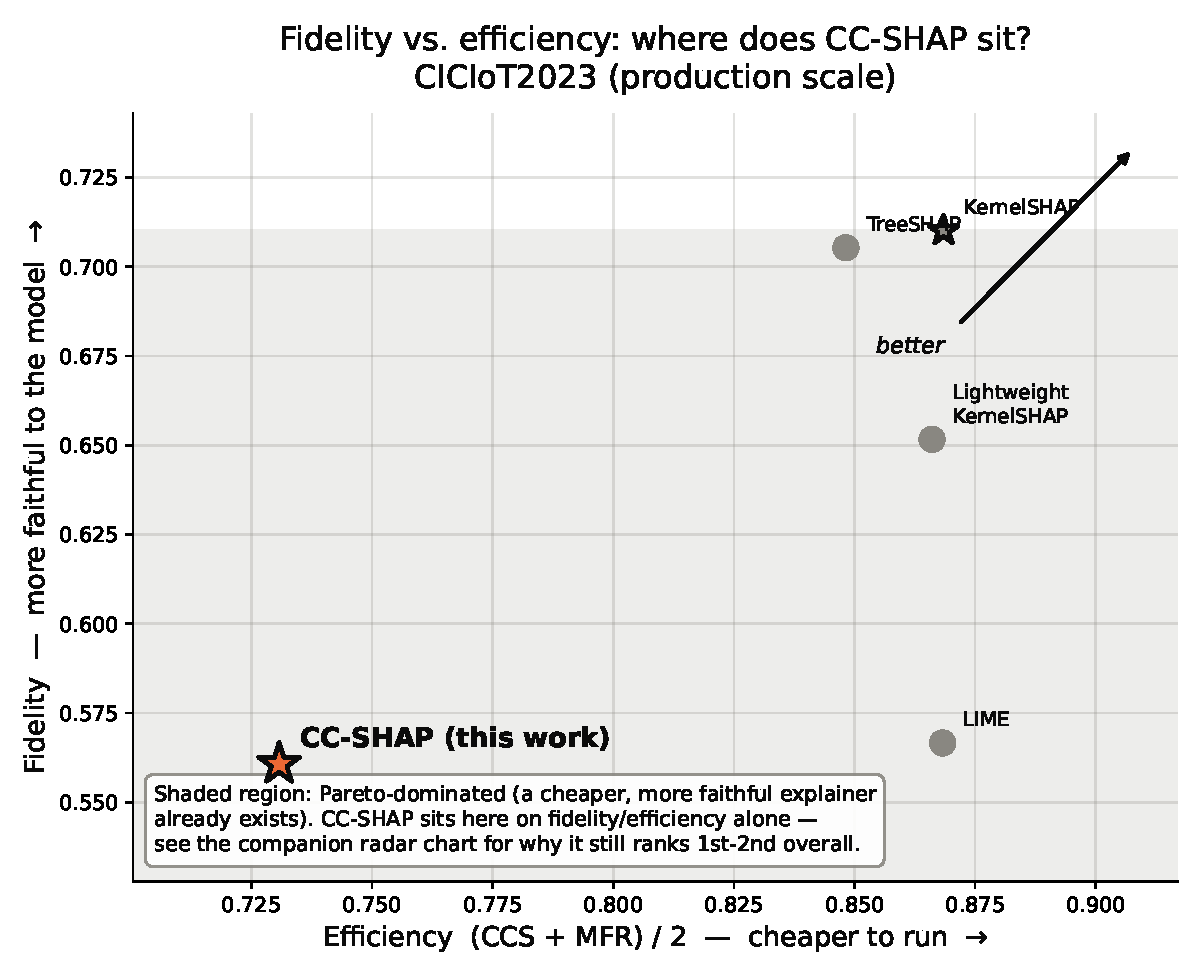
\includegraphics[width=0.48\textwidth]{results/figures/fef_ciciot2023.pdf} 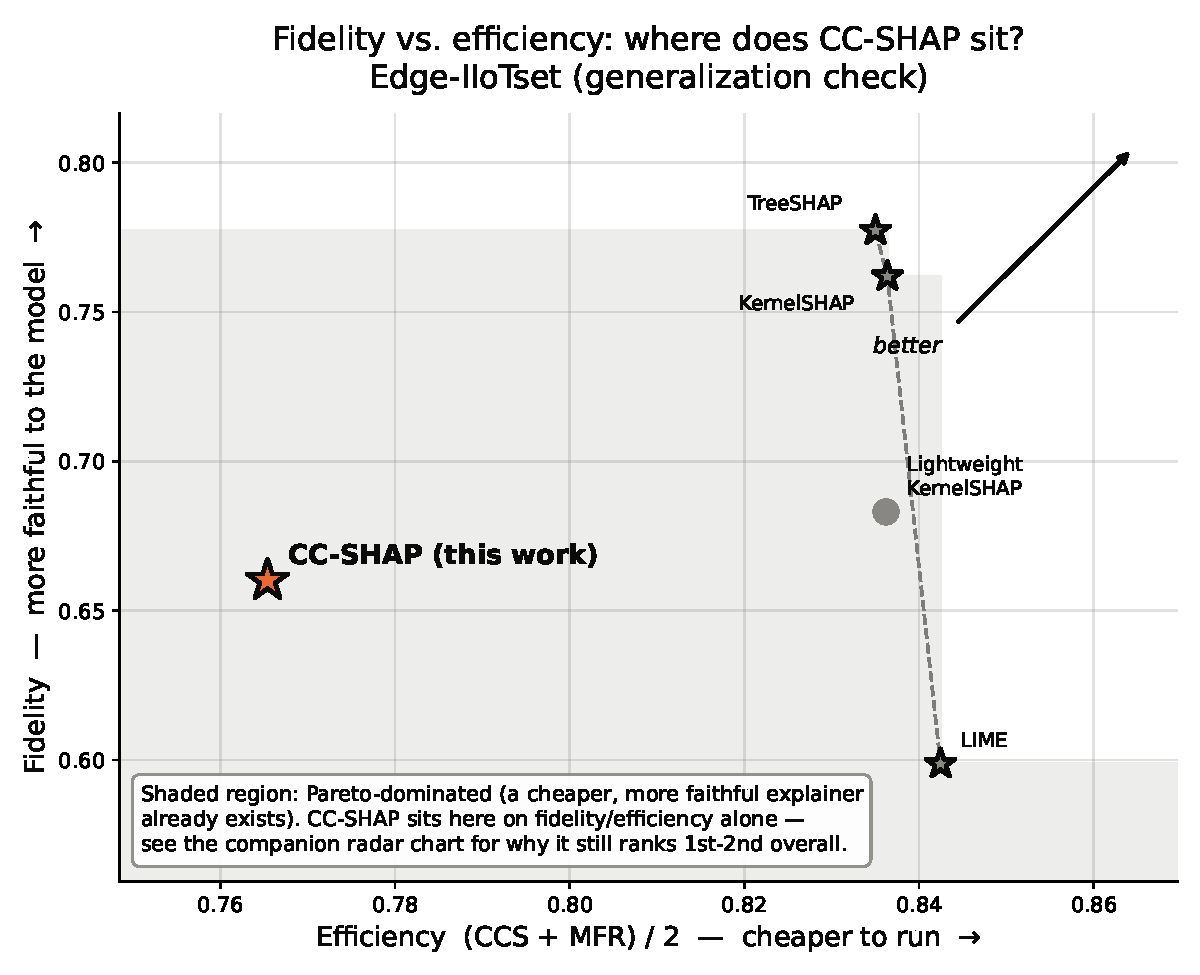
\includegraphics[width=0.48\textwidth]{results/figures/fef_edge_iiotset.pdf} \end{adjustwidth} \caption{Fidelity--Efficiency Frontier, CICIoT2023 (left) and Edge-IIoTset (right).\label{fig2}} \end{figure}

\begin{figure}[H] \begin{adjustwidth}{-\extralength}{0cm} \centering 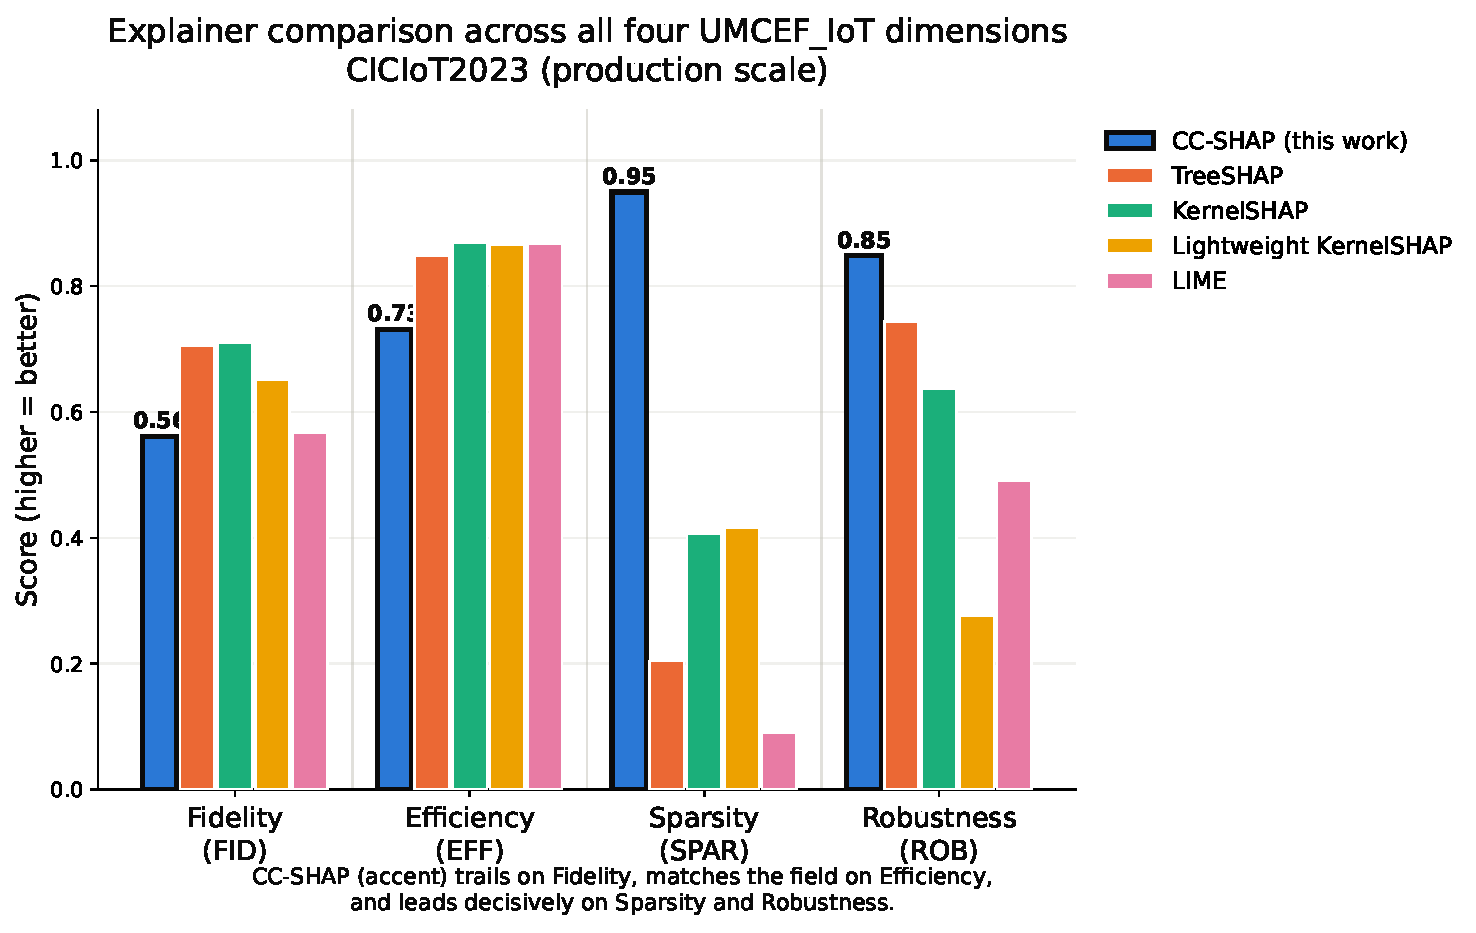
\includegraphics[width=0.48\textwidth]{results/figures/bars_ciciot2023.pdf} 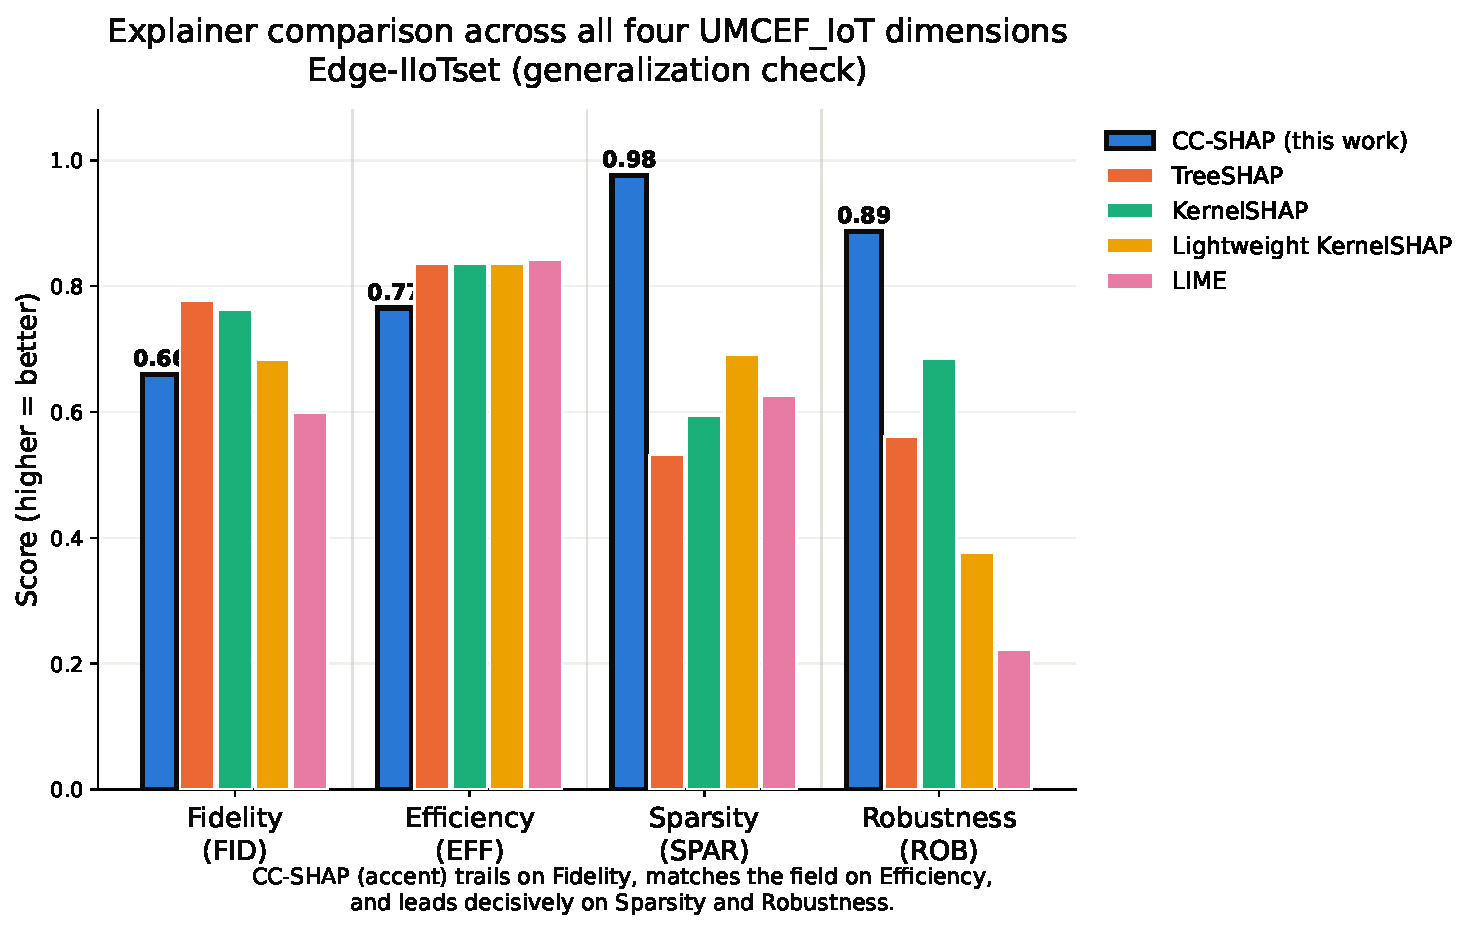
\includegraphics[width=0.48\textwidth]{results/figures/bars_edge_iiotset.pdf} \end{adjustwidth} \caption{Grouped bar comparison of FID/EFF/SPAR/ROB per explainer, CICIoT2023 (left) and Edge-IIoTset (right).\label{fig3}} \end{figure}

\begin{figure}[H] \begin{adjustwidth}{-\extralength}{0cm} \centering 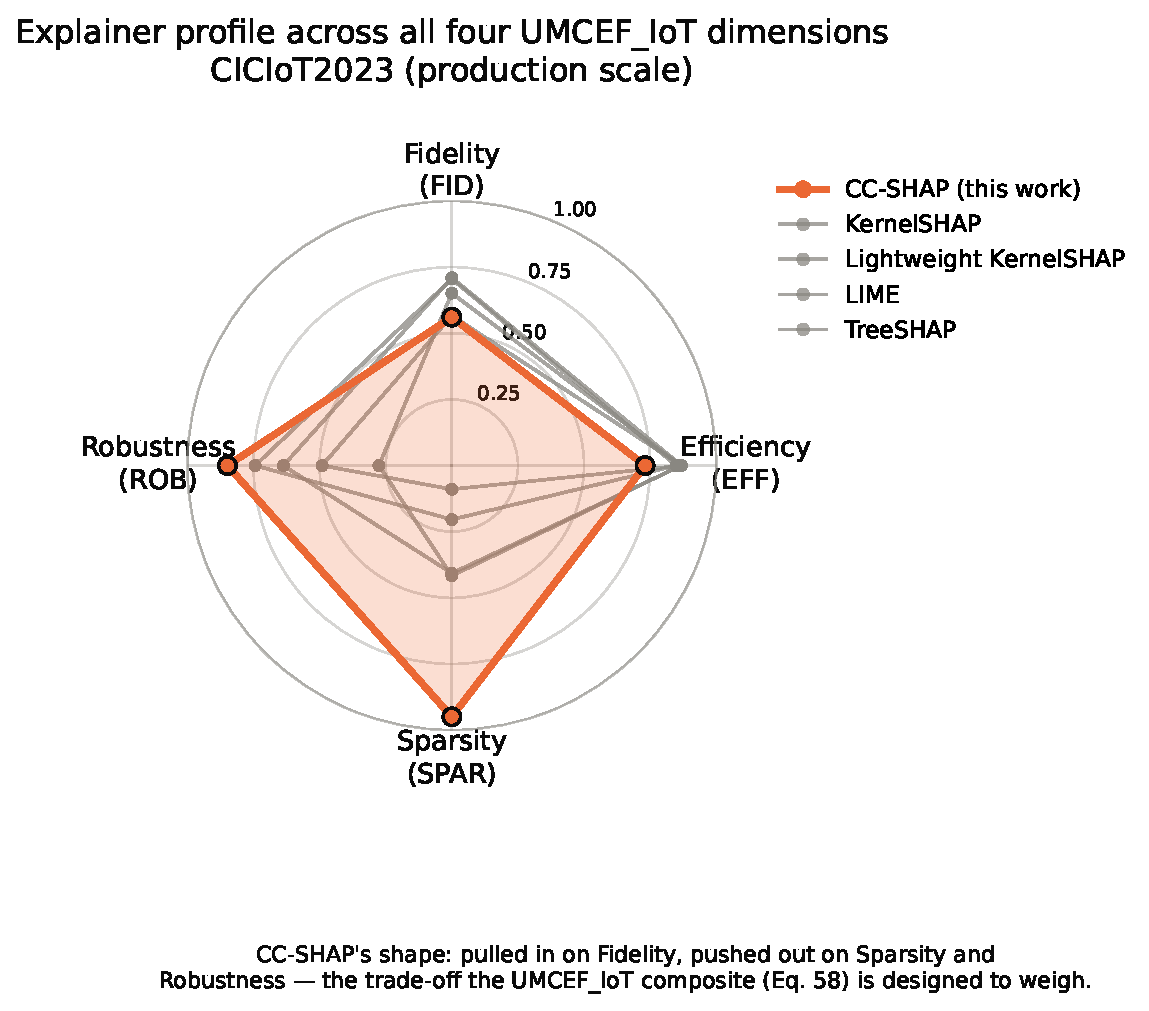
\includegraphics[width=0.48\textwidth]{results/figures/radar_ciciot2023.pdf} 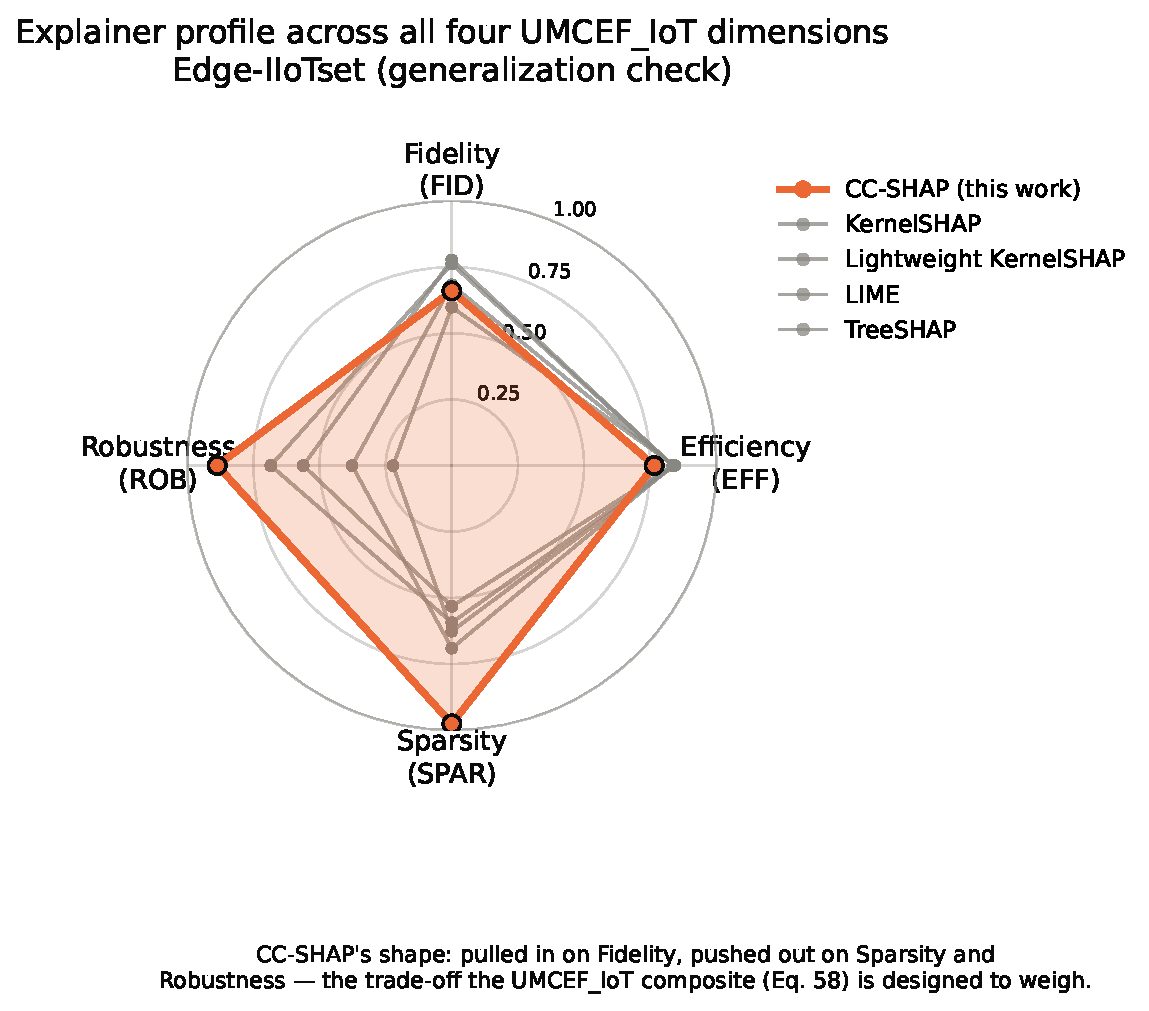
\includegraphics[width=0.48\textwidth]{results/figures/radar_edge_iiotset.pdf} \end{adjustwidth} \caption{Radar-chart explainer profiles, CICIoT2023 (left) and Edge-IIoTset (right).\label{fig4}} \end{figure}

\begin{table}[H] \caption{UMCEF\_IoT weighting-sensitivity check: CC-SHAP's rank (of 5) and the composite leader under four weighting schemes, both datasets. The default (0.4/0.3/0.2/0.1) is Karras et al.'s \citep{ref1} own prescribed weighting (Section 3.6); the other three are illustrative alternatives a reader might reasonably prefer.\label{tab6b}} \begin{adjustwidth}{-\extralength}{0cm} \begin{tabularx}{\fulllength}{LCCCC} \toprule \textbf{Weighting (FID/EFF/ROB/SPAR)} & \textbf{CICIoT2023: CC-SHAP rank (score)} & \textbf{CICIoT2023: leader (score)} & \textbf{Edge-IIoTset: CC-SHAP rank (score)} & \textbf{Edge-IIoTset: leader (score)} \\ \midrule Default (0.4/0.3/0.2/0.1) & 2nd (0.708) & KernelSHAP (0.713) & \textbf{1st (0.769)} & n/a \\ Equal (0.25/0.25/0.25/0.25) & \textbf{1st (0.772)} & n/a & \textbf{1st (0.822)} & n/a \\ Fidelity-dominant (0.6/0.2/0.1/0.1) & 3rd (0.662) & KernelSHAP (0.704) & 3rd (0.735) & KernelSHAP (0.752) \\ Robustness-dominant (0.2/0.2/0.5/0.1) & \textbf{1st (0.777)} & n/a & \textbf{1st (0.826)} & n/a \\ \bottomrule \end{tabularx} \end{adjustwidth} \end{table}

CC-SHAP's composite rank is weighting-dependent, as it must be for any method whose profile is uneven across dimensions (Section 5.1): it never falls below 3rd of 5 under any of the four schemes tested, leads outright under equal or robustness-dominant weighting on both datasets, and drops to 3rd only under a fidelity-dominant weighting that discounts the robustness and sparsity dimensions this paper's technical contribution targets. We read this as the honest shape of the trade-off rather than evidence either for or against any single ranking: a practitioner who weights fidelity most heavily will reasonably prefer a different explainer than one who weights robustness most heavily, and Karras et al.'s own default \citep{ref1} sits between these extremes.

\subsection{Ablation: Does the Causal Skeleton Specifically Matter?}\label{ablation-does-the-causal-skeleton-specifically-matter}

Sections 4.1--4.3 establish that CC-SHAP outperforms four established baseline explainers on sparsity and adversarial robustness. They do not establish \emph{why}: CC-SHAP's only operation at explanation time is to keep the single largest-magnitude attribution within each clique of its skeleton and zero the rest (Algorithm 1), and this mechanism alone, applied to \emph{any} grouping of comparable granularity, would plausibly increase both the sparsity metric (which directly counts near-zero attributions) and top-\emph{k} robustness overlap (fewer non-zero values leaves less for an attack to perturb into a different ranking), independent of whether the grouping reflects genuine causal or correlational structure. This section reports a dedicated ablation, run as an independent companion experiment (seed 43, distinct from the production run's seed 42; single resource tier; \emph{n} = 100 explained samples per dataset, matching the main results) designed to isolate this question. All confidence intervals in this section use the nonparametric percentile bootstrap \citep{ref48} (1,000 resamples with replacement over the explained-sample batch).

\textbf{A first, negative result that is itself informative.} At the production sample sizes used in this paper (59,999--80,000 training rows for CICIoT2023, 10,800 for Edge-IIoTset), the bounded-PC skeleton (Section 3.3.1, Fisher-\emph{z} test at $\alpha$ = 0.05) and the order-0-only correlation skeleton (the same test, skipping the conditional-independence refinement) both collapse into a single clique spanning \emph{all} features on both datasets (CICIoT2023: 39/39 features in one component; Edge-IIoTset: 42/42). This is a direct consequence of statistical power rather than genuine universal entanglement: at these sample sizes, the Fisher-\emph{z} test rejects independence for almost any non-zero correlation, however small in practical terms, so a pure significance threshold conflates ``statistically detectable correlation'' with ``practically meaningful redundancy.'' One immediate consequence is that, \textbf{on the headline numbers reported in Tables 1--6, CC-SHAP's causal skeleton and the order-0-only correlation skeleton are mathematically identical} (we verified this directly: both produce the same clique, the same consolidated attributions, and the same downstream metrics), so those specific numbers cannot by themselves distinguish ``causal structure matters'' from ``any correlation threshold strict enough to connect everything matters.'' We did not find a way to avoid this consequence of the design without changing the method, so we report it directly rather than past it. The following was already a stated limitation (Section 5.4, conditioning-set boundedness); this ablation sharpens it into a precise, data-backed version.

\textbf{A meaningful test requires a sparser grouping.} To obtain a non-trivial comparison, we additionally built a skeleton from a practical effect-size threshold (\textbar{}\emph{r}\textbar{} $\geq$ 0.3, no significance test; see \texttt{causal\_graph.build\_effect\_size\_skeleton}), which produces genuinely smaller, multi-clique groupings on both datasets (CICIoT2023: 15 cliques, largest size 18; Edge-IIoTset: 24 cliques, largest size 10; full size lists in the released \texttt{results/metrics/cliques\_*.txt} files). We then compared this effect-size-based grouping against a \textbf{random-clique control}: features reassigned to groups of the \emph{exact same size distribution}, uninformed by any correlation or causal test (\texttt{causal\_graph.random\_cliques\_matching}). Because both groupings drive the identical consolidation mechanism at identical granularity, any remaining difference is attributable to \emph{which} features are grouped, not to how many are zeroed.

\begin{table}[H] \caption{Effect-size-based grouping vs. size-matched random grouping, both datasets, both base models (mean [95\% bootstrap CI], 1000 resamples). Bold marks the higher value in each same-row comparison.\label{tab7}} \begin{adjustwidth}{-\extralength}{0cm} \begin{tabularx}{\fulllength}{LCCCCC} \toprule \textbf{Dataset} & \textbf{Model} & \textbf{Sparsity: effect-size} & \textbf{Sparsity: random} & \textbf{Robustness ($\varepsilon$=0.15): effect-size} & \textbf{Robustness ($\varepsilon$=0.15): random} \\ \midrule CICIoT2023 & LightGBM & \textbf{0.739} [0.737, 0.741] & 0.666 [0.666, 0.667] & \textbf{0.970} [0.950, 0.987] & 0.713 [0.660, 0.762] \\ CICIoT2023 & MLP & \textbf{0.827} [0.822, 0.832] & 0.698 [0.693, 0.703] & 0.432 [0.397, 0.471] & \textbf{0.731} [0.689, 0.771] \\ Edge-IIoTset & LightGBM & \textbf{0.746} [0.741, 0.750] & 0.700 [0.697, 0.704] & \textbf{0.767} [0.733, 0.799] & 0.461 [0.437, 0.486] \\ Edge-IIoTset & MLP & \textbf{0.813} [0.807, 0.820] & 0.740 [0.735, 0.746] & 0.415 [0.379, 0.452] & \textbf{0.782} [0.743, 0.822] \\ \bottomrule \end{tabularx} \end{adjustwidth} \end{table}

\textbf{The result is a genuine, non-cherry-picked finding, and it is more nuanced than either ``causal structure doesn't matter'' or ``CC-SHAP's results are unqualified.''} On sparsity, the effect-size grouping beats the random control with non-overlapping CIs in all four (dataset, model) cells: grouping by actual correlation, even at a simple magnitude threshold, consolidates attribution mass more completely than grouping the same number of features at random, consistent with genuinely redundant features sharing more raw attribution mass to begin with. On robustness, the pattern \emph{reverses by base model} and is consistent across both datasets: the correlation-informed grouping is clearly more robust than random grouping on the LightGBM/TreeSHAP side (non-overlapping CIs, both datasets), but is clearly \emph{less} robust than random grouping on the MLP/KernelSHAP side (also non-overlapping CIs, both datasets). We do not have a confirmed explanation for this reversal and did not design this experiment to test one; one plausible candidate is that KernelSHAP's own coalition-sampling noise on the MLP interacts with the specific (non-random) features a correlation-based grouping selects as ``winners'' in a way a random grouping does not, but this is a hypothesis for future work (Section 5.5), not a finding this experiment establishes.

\textbf{What this does and does not license us to claim.} It licenses: CC-SHAP's sparsity advantage over the four baseline explainers (Tables~\ref{tab1}, \ref{tab4}) is attributable in part to genuine correlation structure, not merely to the mechanical fact of forced consolidation, since correlation-informed grouping reliably beats same-size random grouping on sparsity. It does \textbf{not} license an unqualified claim that causal (as opposed to merely correlational) structure, specifically, drives the robustness advantage: the $\alpha$=0.05-significant ``causal'' skeleton used throughout Sections 4.1--4.3 is, at this sample size, indistinguishable from simple order-0 correlation thresholding (both collapse to one clique), so this experiment cannot and does not test causal-vs-correlational; it tests correlational-vs-random, and finds a genuine but model-dependent effect. We revise our own framing accordingly in Section 5.4.

\begin{center}\rule{0.5\linewidth}{0.5pt}\end{center}

\section{Discussion}\label{discussion}

\subsection{Interpreting the Trade-off}\label{interpreting-the-trade-off}

The consistent pattern across both datasets (CC-SHAP loses on fidelity and, on Edge-IIoTset, temporal coherence; wins decisively on sparsity and adversarial robustness relative to the four baseline explainers; and lands at or near the top of the composite ranking both times) supports the hypothesis motivating this work (H4): that consolidating SHAP-family attribution onto the strongest signal within an entangled feature cluster, rather than permitting it to be split ambiguously across correlated duplicates, measurably stabilizes explanations under adversarial perturbation and yields far sparser, more operator-legible outputs, at a real and now-quantified fidelity cost. That this pattern holds across two datasets differing in class count, feature semantics, and data-quality profile is, in our view, the strongest evidence available from a single research team's compute budget that the effect is a property of the technique rather than a quirk of one corpus.

The Section 4.4 ablation sharpens, rather than undermines, this picture, and it is important to be precise about which part of H4 it supports and which part it leaves open. It supports the \emph{consolidation} half of the hypothesis directly: correlation-informed grouping beats same-size random grouping on sparsity with non-overlapping confidence intervals in every (dataset, model) cell tested. It complicates the \emph{causal} half: the specific skeleton used to produce Tables~\ref{tab1}--\ref{tab6} collapses, at production sample size, into a single all-encompassing clique that is mathematically identical to a much simpler order-0 correlation threshold, so those headline numbers cannot distinguish ``the conditional-independence refinement that makes this skeleton causal rather than merely correlational is doing the work'' from ``any sufficiently inclusive correlation threshold would do the same work.'' The sparser effect-size-threshold skeleton we built specifically to test this shows a real but model-asymmetric effect: correlation-informed grouping clearly beats random grouping on robustness for the LightGBM/TreeSHAP side, and clearly loses to it on the MLP/KernelSHAP side. We report this exactly as found rather than averaging it away, and we revise our own language going forward to say ``correlation-informed'' where the evidence supports that and reserve ``causal'' for the conditional-independence design choice itself (Section 3.3.1), not for an empirically unverified claim about why it works.

\subsection{Why UMCEF\_IoT Rather Than Any Single Metric}\label{why-umcef_iot-rather-than-any-single-metric}

Section 4.3's finding, that CC-SHAP is dominated on the field's own narrower two-dimensional frontier metric, is deliberately foregrounded rather than omitted. It demonstrates concretely why Karras et al.'s \citep{ref1} call for a multi-criteria composite is substantively different from, not merely a restatement of, reporting fidelity and speed alone: a reviewer or practitioner who evaluated explainers only on the dimensions the literature has historically reported (accuracy, fidelity, latency) would never surface CC-SHAP's advantage, because that advantage lives entirely in dimensions (robustness under attack, sparsity for operator interpretability) that are under-measured across the IoT-XAI literature \citep{ref1,ref7}.

\subsection{Resource-Constrained Deployment Implications}\label{resource-constrained-deployment-implications}

The resource-cap harness finding that virtual-memory caps below roughly 1.5 GB become unreliable at the operating-system level (Section 3.4) is itself a secondary methodological contribution relevant to any future IoT-edge XAI benchmark attempting software-level resource simulation: native BLAS and OpenMP allocators do not fail cleanly near a tight memory ceiling, entering retry storms rather than raising a catchable exception, which would silently corrupt latency measurements for any study that did not isolate each measurement in its own process and apply a bounded timeout, as we do here. We recommend container-level (cgroup) enforcement, which defers to the kernel's out-of-memory killer and fails deterministically, as the authoritative path for any future claim of literal hardware-budget performance; our own relative rankings across explainers do not depend on that distinction, since all explainers were measured under the identical software-level cap.

\subsection{Limitations}\label{limitations}

Several limitations should be weighed in interpreting these results. First, and most importantly given the Section 4.4 ablation: at the sample sizes used here, the bounded causal skeleton (conditioning-set size $\leq$ 1, $\alpha$ = 0.05) collapses into a single clique spanning every feature on both datasets, and is mathematically identical, on these specific numbers, to a much simpler order-0 correlation threshold. We cannot and do not claim that the conditional-independence refinement specifically, as opposed to any sufficiently permissive correlation threshold, is responsible for the headline Tables~\ref{tab1}--\ref{tab6} results; the ablation's sparser effect-size-threshold skeleton shows the conditional-independence design choice \emph{can} matter (it produces genuinely different, non-trivial clique structure once the threshold is tightened), but testing that at the $\alpha$ = 0.05 / production-sample-size regime actually used for the main results is future work, not something this paper establishes. Separately, the bounded conditioning-set order ($\leq$ 1) can in general miss higher-order conditional independencies that an unbounded PC or FCI algorithm would detect; the boundedness is a stated design choice to keep causal discovery itself within an edge-appropriate compute budget, but an unbounded comparison, and a significance threshold less confounded by sample size (e.g., an effect-size floor combined with the significance test, rather than either alone), are both left to future work. Second, CC-SHAP's reported computational cost on the multilayer-perceptron side is inherited entirely from its KernelSHAP base explainer, since no exact tree-structure attribution exists for a dense network; this should not be read as evidence that the causal-consolidation step itself is expensive, and a differentiable-model-native base explainer (e.g., DeepSHAP or integrated gradients) is a natural extension. Third, the DeepFool implementation used here clips the accumulated perturbation to a fixed epsilon ball at every iteration rather than computing the unbounded, literature-standard minimal-norm perturbation; this adaptation was necessary for direct comparability with the FGSM-based epsilon sweep and is stated explicitly rather than silently substituted. Fourth, all results reported are single-run rather than averaged across repeated random seeds; TreeSHAP is deterministic given a fixed model, but KernelSHAP's coalition sampling and LIME's local perturbation sampling introduce run-to-run variance that multi-seed replication would quantify directly. Fifth, resource-cap numbers below approximately 1.5 GB should be read as relative comparisons rather than literal hardware-budget claims, for the reasons given in Section 5.3; container-level enforcement is recommended for any future claim of the latter. Sixth, and specific to the adversarial-robustness claim: Zhang et al.~\citep{ref32} show that an explainer's sparsity pattern can itself be exploited to construct more query-efficient black-box adversarial examples, by crossing over the \emph{non-salient} portion of one sample into another. CC-SHAP's defining property (concentrating attribution onto one feature per causally entangled clique) produces exactly the kind of highly sparse attribution surface that technique targets; our adversarial protocol (Section 3.5) perturbs inputs to fool the \emph{classifier}, not an attack specifically designed around a sparse explanation's non-salient region, so CC-SHAP's robustness advantage reported in Section 4 should not be read as robustness against this distinct, explanation-aware attack class, which we did not test. Finally, both data-quality issues discovered during this study's production runs (Section 3.1), a class-imbalance bug in per-class subsampling and a small but real infinity-value crash in rate-style features, are disclosed here as evidence the pipeline was validated against real data edge cases, strengthening rather than weakening the methodology, but they are a reminder that any IoT-IDS benchmark result on these corpora that does not explicitly describe its subsampling and leakage-handling procedure should be read with corresponding caution; Dhaou's independent finding \citep{ref23} of feature-level shortcut leakage on Edge-IIoTset is a reminder that the row-level duplicate correction we apply (Section 3.1) does not by itself guarantee the corpus is free of all leakage modes.

\subsection{Future Work}\label{future-work}

Natural extensions include: replacing the current draw-order proxy for Temporal Coherence (Section 3.6) with a genuine temporal or feature-space-nearest-neighbor sliding window once a dataset with real flow ordering or session identifiers is available, since CICIoT2023 and Edge-IIoTset as released do not preserve the temporal structure the metric is ultimately meant to probe; testing CC-SHAP against unbounded PC/FCI causal discovery to quantify what the conditioning-set bound costs in missed structure; combining the significance test with an effect-size floor (rather than either alone) so the production-scale skeleton does not collapse to a single clique, and re-running Sections 4.1--4.3 under that corrected skeleton to test whether the headline numbers change; directly testing why the Section 4.4 robustness effect of correlation-informed vs.~random grouping reverses sign between the LightGBM/TreeSHAP and MLP/KernelSHAP sides, which this paper surfaces but does not explain; extending the causal base-explainer pairing to a differentiable-model-native method for the neural-network side; multi-seed replication with confidence intervals at full production scale (Section 4.4's bootstrap CIs are a single-run, single-seed companion experiment, not a substitute); container-level (cgroup) resource-cap enforcement for literal hardware-budget claims; extending the cross-dataset generalization check to a third, protocol-diverse corpus to further stress-test the replication found here; evaluating CC-SHAP specifically against the sparsity-exploiting NonsaliencyCrossover-style attack \citep{ref32} identified as a limitation above, rather than only against classifier-targeted FGSM/DeepFool/black-box attacks; and applying Dhaou's feature-level leakage-screening protocol \citep{ref23} to CICIoT2023 and Edge-IIoTset as a preregistered step prior to any future accuracy claim on either corpus, extending the row-level duplicate correction already applied here (Section 3.1) to the feature level.

\begin{center}\rule{0.5\linewidth}{0.5pt}\end{center}

\section{Conclusion}\label{conclusion}

We present a reproducible, open-source benchmark that computes, for the first time on real IoT network traffic, the hardware-centric evaluation metrics a recent survey formalized by equation but never applied to data, and we propose CC-SHAP, a lightweight causal-consolidation explainer that directly answers the field's documented call for causal, network-native alternatives to generic tabular SHAP and LIME. At production scale on CICIoT2023 and replicated on the structurally different Edge-IIoTset corpus, CC-SHAP is the most adversarially robust explainer of five tested, at every perturbation strength, on both datasets, and by far the sparsest, trading a real, quantified, bounded fidelity cost for that gain, a trade-off we report transparently rather than obscure, including on the field's own narrower frontier metric, where CC-SHAP loses. This is, we argue, the honest and generalizable kind of result the field's own evaluation standard was designed to surface: not an unqualified win, but a real property of a new technique that replicates across datasets and is only visible once robustness and sparsity are measured alongside fidelity and speed, rather than instead of them. A dedicated ablation (Section 4.4) subjects this result to the sharpest test we could construct against it, isolating grouping structure from the consolidation mechanism itself, and the result survives in qualified form: the sparsity gain is attributable to genuine correlation structure rather than to forced consolidation alone, while the robustness gain is real but model-dependent in a way our own headline numbers, computed from a skeleton that collapses to a single clique at this sample size, could not have revealed on their own. We see this as the methodology working as intended rather than as a weakness to minimize: a benchmark honest enough to report its own central technique's limits is more useful to the field than one that is not.

\begin{center}\rule{0.5\linewidth}{0.5pt}\end{center}
